Following the work of \cite{Brosse18tULA}, we aim to quantify the accuracy of these methods by finding the first and second moments of known distributions. Then, comparing the error between the generated value and the true value will give a first indication on the accuracy of the scheme. Beginning with the original code associated with \cite{Brosse18tULA}\footnote{Available at \url{https://github.com/nbrosse/TULA}}, we initially optimised the code then aimed to reproduce the results they found. 

\subsection{Testing Potentials}
For the purposes of testing, four qualitatively different potentials have been made available within our program. These are: Gaussian, Double Well, Rosenbrock function and Ginzburg-Landau model. We note that these, save for Gaussian, are non-convex.

Any of the above potentials may also be scaled by \textit{temperature} $T$. That is, having chosen a potential function $U$ and a temperature $T$, the true distribution to be sampled from will be
\[\pi(x) = e^{-\frac{U(x)}{T}}.\]
This is common in the molecular dynamics literature and is also useful in MCMC to find modes of distributions more quickly, a technique known as tempering.

Figure \ref{fig:tamedStep} shows how taming prevents divergence even at higher step sizes, where the untamed algorithms would diverge. Figure \ref{fig:doubleWell_moment} compares first and second moments of the double well distribution in 100 dimensions after running the methods for \(10^5\) iterations and with a stepsize of \(h=0.1\). Note that \texttt{ULA} and \texttt{HOLA} diverge and produce no useful samples. Theoretically, the first moment of this distribution is 0, and the second moment is around 0.104 in 100 dimensions. It can be seen that at this larger step size, the taming is causing an overestimation of the second moment for \texttt{tULA,tLM} and \texttt{tHOLA}. Adjusting the taming to a coordinatewise function is reducing the issue. This a similar phenomena to that seen in Section \ref{sec:stiff}. Figure \ref{fig:timedRun} takes a different approach. Rather than running each algorithm for a fixed number of iterations, we instead let each scheme run for 10 seconds. It can be seen that \texttt{tHOLA} has a much higher range of error when stepsize is low. This is because each iterate takes much longer than the other methods, resulting in an order of magnitude fewer samples being produced in 10 seconds. This is due to the algorithm involving the multiplication of large matrices, a costly computation. When the stepsize is increased the Metroplised algorithms seem to perform worst. It is unclear why this should be the case. Once again \texttt{ULA} and \texttt{LM} diverge.

\begin{figure}
\centering
  \begin{minipage}[b]{0.32\textwidth}
  \centering
    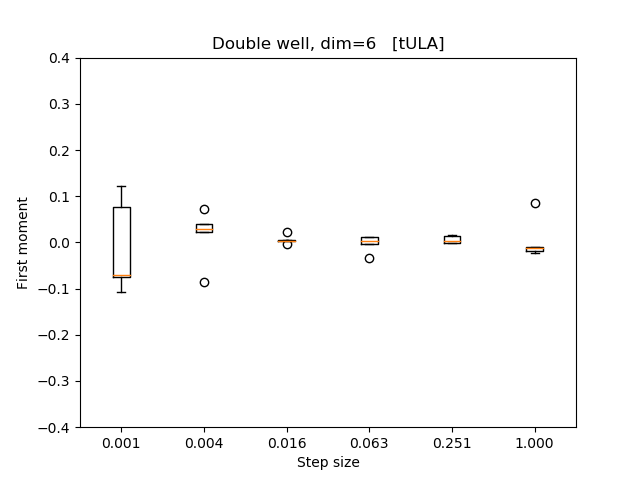
\includegraphics[width=\textwidth]{Figures/tula_fm.png}
  \end{minipage} %
  \begin{minipage}[b]{0.32\textwidth}
  \centering
    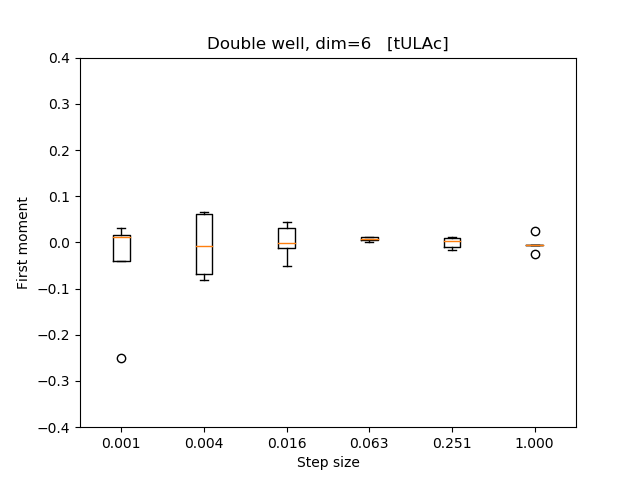
\includegraphics[width=\textwidth]{Figures/tulac_fm.png}
  \end{minipage} %
  \begin{minipage}[b]{0.32\textwidth}
  \centering
    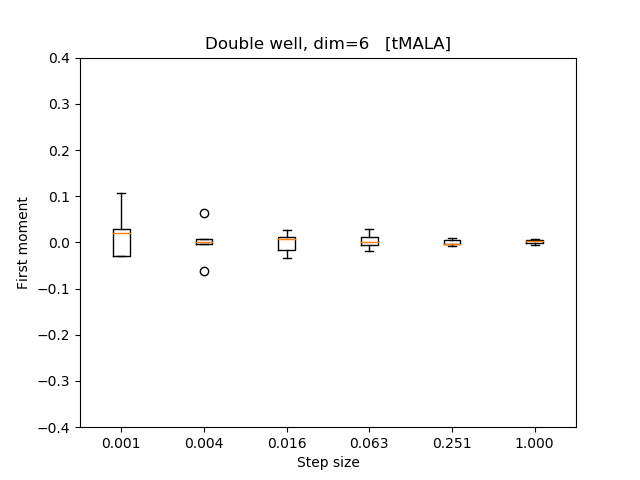
\includegraphics[width=\textwidth]{Figures/tmala_fm.png}
  \end{minipage}
   \caption{Comparison of \texttt{tULA}, \texttt{tULAc} and \texttt{tMALA} for the first moment evolving as a function of step size.}
   \label{fig:tamedStep}
\end{figure}

\begin{figure}
\centering
  \begin{minipage}[b]{0.85\textwidth}
  \centering
    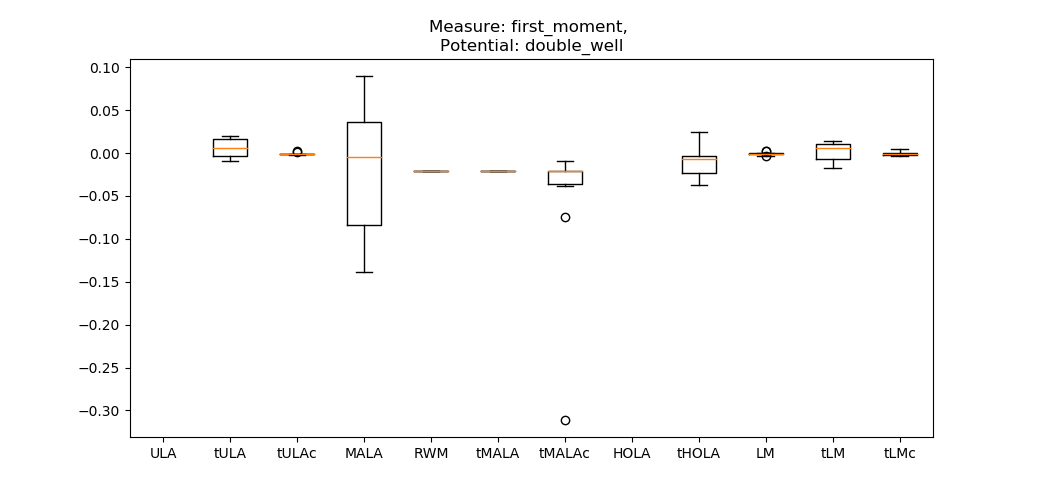
\includegraphics[width=\textwidth]{Figures/doublewell_0_1_10_5samp_100dFirstMoment.png}
  \end{minipage}\\ %
  \begin{minipage}[b]{0.85\textwidth}
  \centering
    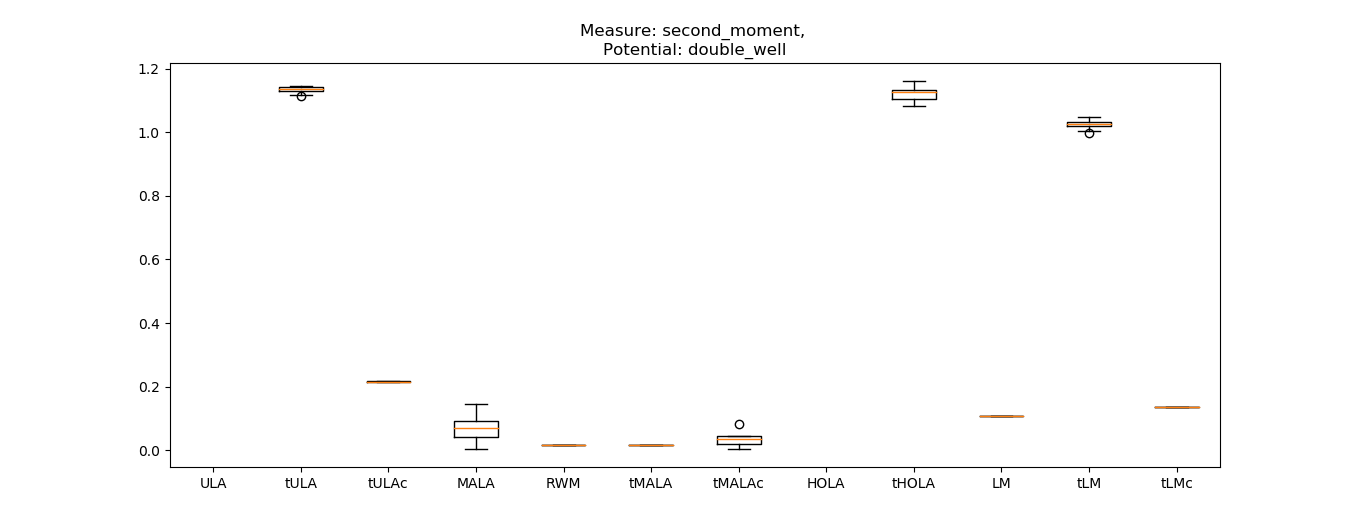
\includegraphics[width=\textwidth]{Figures/secondmoment_double_well_100d_10_5samp.png}
  \end{minipage} %
  \caption{Comparison of first (top) and second (bottom) moments of the double well distribution in 100 dimensions after running the methods for \(10^5\) iterations and with a stepsize of \(h=0.1\). Note that \texttt{ULA} and \texttt{HOLA} diverge and produce no useful samples.}
  \label{fig:doubleWell_moment}
  \end{figure}
  
  \begin{figure}
\centering
  \begin{minipage}[b]{0.47\textwidth}
  \centering
    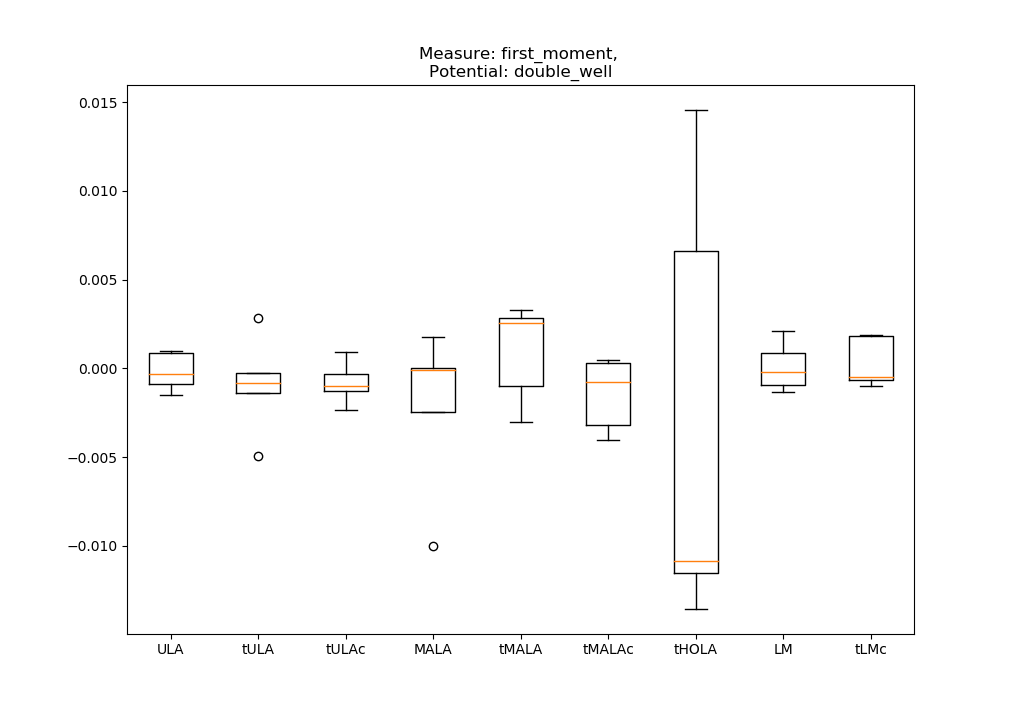
\includegraphics[width=\textwidth]{Figures/10sBoxPlot1moment100dim001step.png}
  \end{minipage} %
  \begin{minipage}[b]{0.47\textwidth}
  \centering
    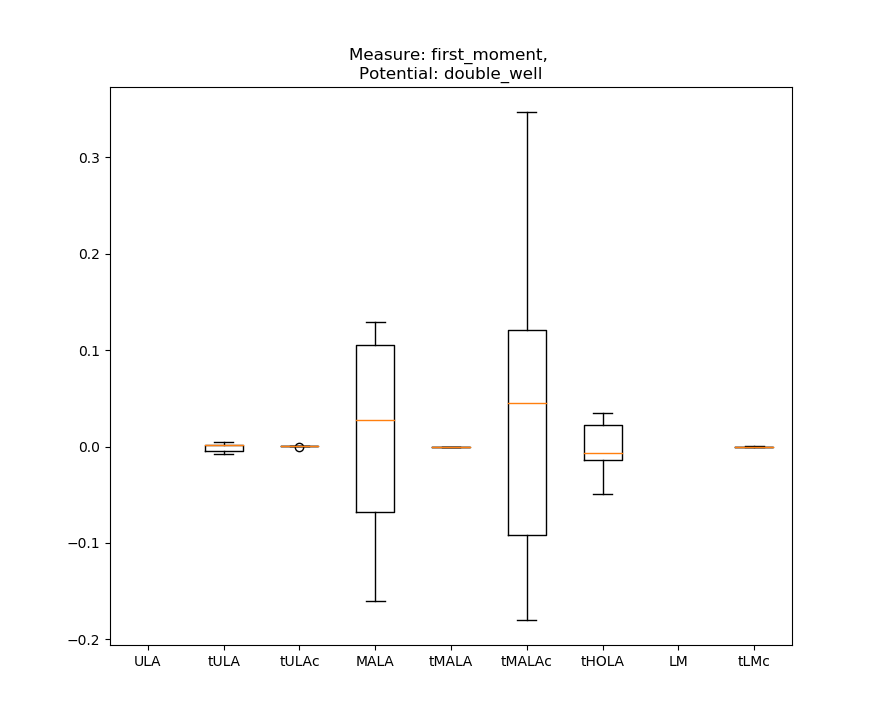
\includegraphics[width=\textwidth]{Figures/10sBoxPlot1moment100dim01step.png}
  \end{minipage} %
  \caption{Comparison of methods when given 10 seconds to run at \(h=0.01\) (left) and \(h=0.1\) (right). Note that \texttt{ULA} and \texttt{LM} both diverge when the stepsize is too high.}
  \label{fig:timedRun}
  \end{figure}